% Created 2017-07-06 Thu 09:00
\documentclass[a4paper]{article}
\usepackage[utf8]{inputenc}
\usepackage[T1]{fontenc}
\usepackage{fixltx2e}
\usepackage{graphicx}
\usepackage{longtable}
\usepackage{float}
\usepackage{wrapfig}
\usepackage{rotating}
\usepackage[normalem]{ulem}
\usepackage{amsmath}
\usepackage{textcomp}
\usepackage{marvosym}
\usepackage{wasysym}
\usepackage{amssymb}
\usepackage{hyperref}
\tolerance=1000
\usepackage{minted}
\usepackage[margin=0.8in]{geometry}
\usepackage{amssymb,amsmath}
\usepackage{fancyhdr} %For headers and footers
\pagestyle{fancy} %For headers and footers
\usepackage{lastpage} %For getting page x of y
\usepackage{float} %Allows the figures to be positioned and formatted nicely
\floatstyle{boxed} %using this
\restylefloat{figure} %and this command
\usepackage{hyperref}
\hypersetup{urlcolor=blue}
\usepackage{minted}
\setminted{frame=single,framesep=10pt}
\chead{}
\rhead{\today}
\cfoot{}
\rfoot{\thepage\ of \pageref{LastPage}}
\author{Nathan Hughes (\href{mailto:nah31@aber.ac.uk}{nah31@aber.ac.uk})}
\date{\today}
\title{Genetics Dictonary}
\hypersetup{
  pdfkeywords={},
  pdfsubject={},
  pdfcreator={Emacs 24.5.1 (Org mode 8.2.10)}}
\begin{document}

\maketitle
\maketitle
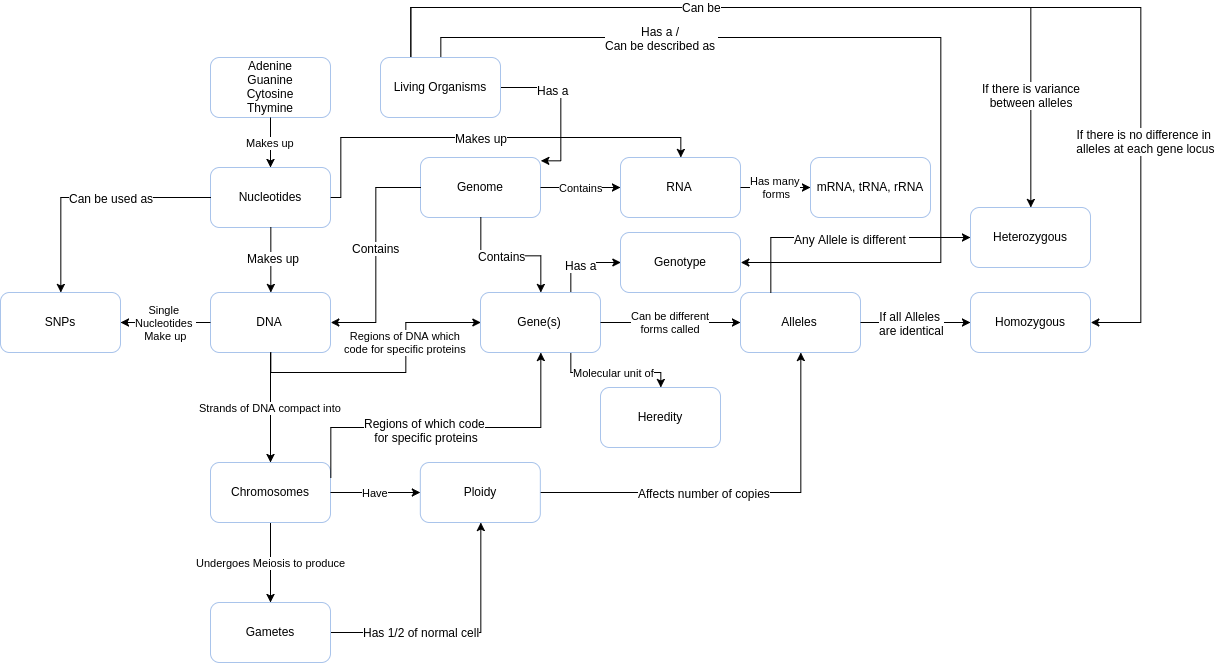
\includegraphics[width=.9\linewidth]{./images/biologyTree.png}
\clearpage
\tableofcontents
\clearpage


\section{QTL}
\label{sec-1}
\begin{itemize}
\item Quantitative Trait Locus
\item See \href{./QTL.pdf}{QTL Notes}
\end{itemize}

\section{Phenotype}
\label{sec-2}
\begin{itemize}
\item The physical manifestation of a trait
\end{itemize}

\section{Genotype}
\label{sec-3}
\begin{itemize}
\item The genetic makeup of an individual organism
\end{itemize}

\section{Nucleotide}
\label{sec-4}
\begin{itemize}
\item Building blocks of nucleic acids
\item Basis of constructing DNA
\end{itemize}

\section{SNPs}
\label{sec-5}
\begin{itemize}
\item Single*nucleotide polymorphism
\item Is a region of DNA which varies
\item i.e. C*G changing to a T*A in one specific place
\item Can be found through the PCR process (amongst others)
\end{itemize}

\section{DNA}
\label{sec-6}
\begin{itemize}
\item Deoxyribonucleic acid
\item Is a molecule that carries all genetic instructions of a living organism
\end{itemize}

\section{Chromosome}
\label{sec-7}
\begin{itemize}
\item is a DNA molecule that has been packaged into thread-like structures
\item Each chromosome is made up of DNA tightly coiled many times around proteins called histones
\item Is visible under microscope when cells are dividing.
\item Linear arrangements of condensed DNA
\end{itemize}

\section{Ploidy}
\label{sec-8}
\begin{itemize}
\item The number of sets of chromosomes in a cells
\item The possible number of alleles for autosomal and pseudoautosomal genes
\end{itemize}

\section{Gene}
\label{sec-9}
\begin{itemize}
\item A region of DNA
\item Made up of nucleotides
\item Sometimes called locus of DNA
\item Is the molecular unit of heredity
\end{itemize}

\section{Genome}
\label{sec-10}
\begin{itemize}
\item Encompasses DNA, RNA and mitochrondria/chroloplasts of an organism.
\end{itemize}

\section{Homozygous}
\label{sec-11}
\begin{itemize}
\item An gene is said to be homozygous  when identical alleles of the gene are present on all chromosomes
\item Homozygous*dominant for a trait carries multiple copies for the dominant trait
\end{itemize}

\section{Heterozygous}
\label{sec-12}
\begin{itemize}
\item A gene is said to be heterozygous when at a gene locus there is two different alleles (copies of the same gene)
\end{itemize}

\section{Homologous Chromosomes}
\label{sec-13}
\begin{itemize}
\item Are the set made from both parents during meiosis
\item Homologs have the same genes in the same loci where they provide points along each chromosome
\item They enable a pair of chromosomes to align correctly before separating during meiosis
\item Fig. 1 Illustrates this process
\end{itemize}

\begin{figure}[htb]
\centering
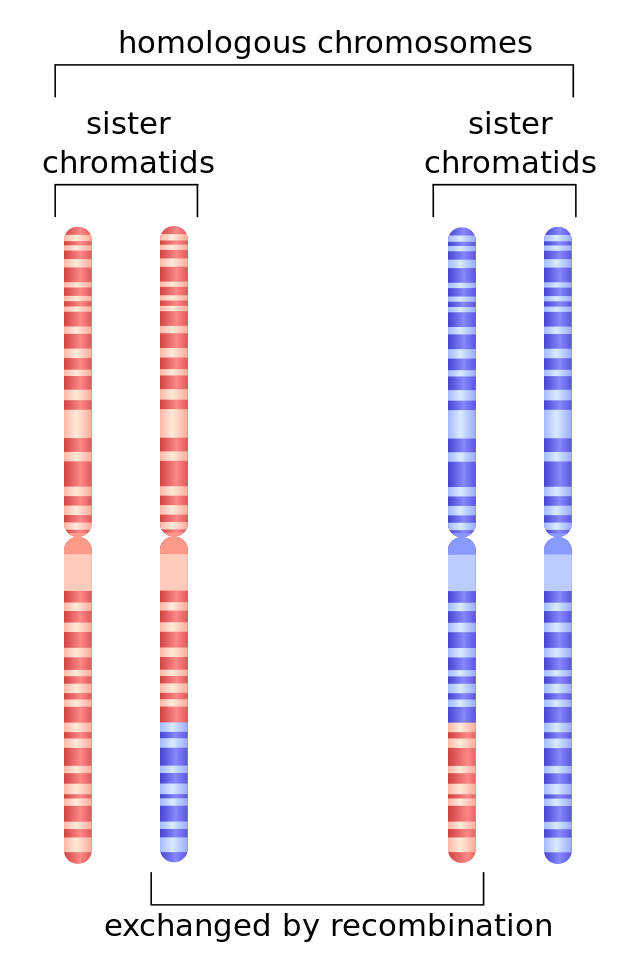
\includegraphics[width=0.2\textwidth,height=0.3\textwidth]{./images/meiosis.png}
\caption{\label{fig:Meiosis}During the process of meiosis, homologous chromosomes can recombine and produce new combinations of genes in the daughter cells.}
\end{figure} 

\section{Recombinaton}
\label{sec-14}
\begin{itemize}
\item Is a process by which pieces of DNA are borken and recombined to produce new combinations of alleles
\item In eukaryotic cells, this typically happens during meiosis
\item Genes that are located further apart on the same chromosome have a greater chance of undergoing recombination
\end{itemize}


\section{Meiosis}
\label{sec-15}
\begin{itemize}
\item Is a form of cell division that produces gametes
\item During the first phase of meiosis, the homologous pairs of parental chromosomes can overlap and temporally fuse, causing a crossover
\end{itemize}

\section{Gametes}
\label{sec-16}
\begin{itemize}
\item These are (generally(don't ask)) haploid cells 
\begin{itemize}
\item i.e. have one set of paternal chromosomes
\end{itemize}
\item Used in sexual reproduction
\end{itemize}

\section{Gametogenesis}
\label{sec-17}
\begin{itemize}
\item Is the biological process by which diploid or haploid cells undergo cell division
\item Produces Gametes
\end{itemize}

\section{Backcross}
\label{sec-18}
\section{Alleles}
\label{sec-19}
\section{Chromosomes}
\label{sec-20}
\section{Recombination}
\label{sec-21}
\section{Progeny}
\label{sec-22}
\section{Transcription}
\label{sec-23}
\section{Candidate gene}
\label{sec-24}
\section{Mendelian inheritance}
\label{sec-25}
\begin{itemize}
\item Is a type of inheritance that follows the laws of Gregor Mendel
\item Fig. 2 Illustrates dominant and recessive phenotypes
\item Fig. 3 Illustrates the law of independent assortment
\item The Law of Dominance states that recessive alleles will always be masked by dominant alleles. Therefore, a cross between a homozygous dominant and a homozygous recessive will always express the dominant phenotype, while still having a heterozygous genotype.
\end{itemize}
\begin{figure}[htb]
\centering
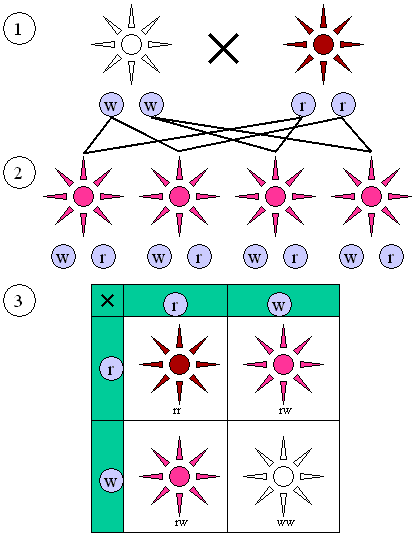
\includegraphics[width=0.2\textwidth,height=0.3\textwidth]{./images/mendel.png}
\caption{\label{fig:Mendel}(1) Parental generation. (2) F1 generation. (3) F2 generation. Dominant (red) and recessive (white) phenotype look alike in the F1 (first) generation and show a 3:1 ratio in the F2 (second) generation.}
\end{figure}

\begin{figure}[htb]
\centering
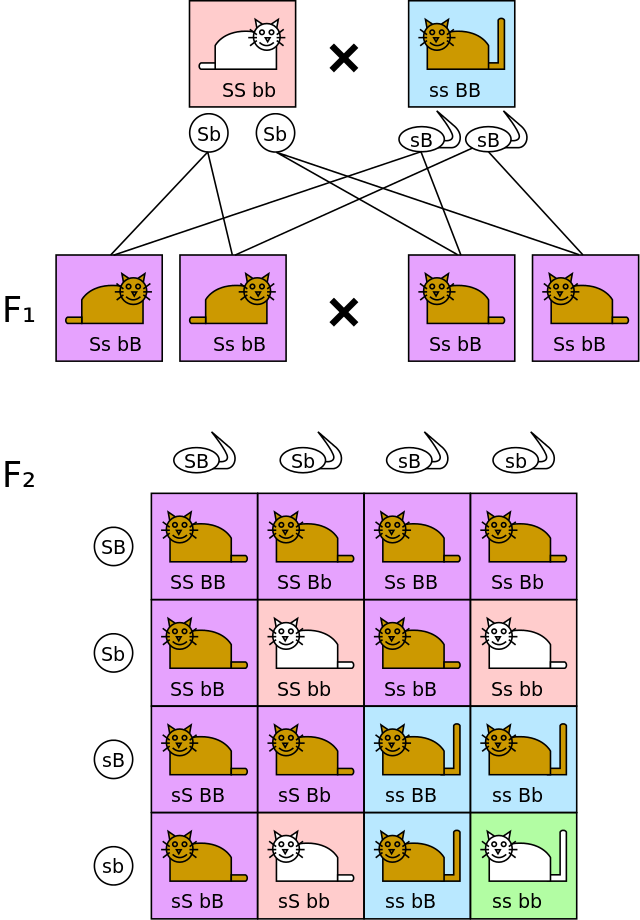
\includegraphics[width=0.2\textwidth,height=0.3\textwidth]{./images/mendel2.png}
\caption{\label{fig:Mendel2}The phenotypes of two independent traits show a 9:3:3:1 ratio in the F2 generation. In this example, coat color is indicated by B (brown, dominant) or b (white), while tail length is indicated by S (short, dominant) or s (long). When parents are homozygous for each trait (SSbb and ssBB), their children in the F1 generation are heterozygous at both loci and only show the dominant phenotypes (SsbB). If the children mate with each other, in the F2 generation all combinations of coat color and tail length occur: 9 are brown/short (purple boxes), 3 are white/short (pink boxes), 3 are brown/long (blue boxes) and 1 is white/long (green box).}
\end{figure}

\section{Heritability}
\label{sec-26}
% Emacs 24.5.1 (Org mode 8.2.10)
\end{document}